% !TeX spellcheck = en_US
\addscenariosection{1}{Cooperative Scenario}{Close to enemies}{\images/balistic.png}

\begin{multicols}{2}

\textbf{Author:} Kelghor

\textbf{Version:} 1.5

\textbf{Source:} \href{https://discord.com/channels/740870068178649108/1313651865648369725}{Archon Studio Discord}

\textit{``Sir! The raiders are at our gates!''}

\textit{``Sound the warhorn! We'll drive them back as always!'' you command, and go to defend the city. Just as you have done many times before. Such is the harsh life of the border clans, where wars and skirmishes with neighboring rivals never truly end. Fortunately, your alliance remains strong, and you know your back is covered.}

\textit{Therefore, the time has come to end the long-standing wars and crush your enemies like a bug once and for all!}

\subsection*{\MakeUppercase{Scenario Length}}

This Scenario is played over 7 Rounds.

\subsection*{\MakeUppercase{Player Setup}}

\textbf{Player Count:} 1-6

\textbf{Starting Resources:} 14 \svg{gold}, 5 \svg{building_materials}, 2 \svg{valuables}

\textbf{Starting Income:} 10 \svg{gold}, 2 \svg{building_materials}, 0 \svg{valuables}

\textbf{Starting Units:}
\begin{itemize}
  \item  1 × A Few \svgunit{bronze} Units of your choice
\end{itemize}

\textbf{Town Buildings:} \svgunit{bronze} Dwelling.

\textbf{Map Tile Pool:} Take $P$ × random Far (II–-III) Map Tiles to form a shared pool, where $P$ equals the number of players. None of these tiles may contain a Settlement.

\subsection*{\MakeUppercase{Map Setup}}

Take the following Map Tiles and arrange them as shown in the Scenario map layout.
Place Far (II--III) Map Tiles with Settlements that match your Faction's Towns. Mark these with a colored Cube (see example).

\begin{itemize}
  \item $P$ × Starting (I) Map Tile.
  \item $P$ × Far (II--III) Map Tile with Settlement of same Faction as players Towns.
  \item 2$P$ × Far (II--III) Map Tile - must not contain Tiles with Settlements.
\end{itemize}

\textit{Optional: You can distribute random pieces and covered pieces on the map so that they match your Faction's basic terrain.}

\subsection*{\MakeUppercase{AI Hero Setup}}

Prepare an AI Deck for Settlement defenders.

\textbf{Settlement defenders Deck:} 1 × Attack Card, 1 × Defense Card, 1 × Spell Card

\textbf{Settlement defenders Spell Deck:} 1×Magic Arrow

\subsection*{\MakeUppercase{Victory Conditions}}
Conquer all Settlements by any player.

\subsection*{\MakeUppercase{Defeat Conditions}}

\begin{itemize}
  \item Any player lose his town.
  \item All settlements are not owned by any player at the end of 7th turn.
\end{itemize}

\subsection*{\MakeUppercase{Additional Rules}}

\begin{itemize}
  \item At any time, Players can spend their Building Token to perform the same actions as if they visited a Trading Post.
  \item When defending the town, and your Hero is not here, you can still use your Units (for free).
  \item Each settlement is defend by clans Settlement defenders. (see below)
\end{itemize}

\subsection*{\MakeUppercase{Timed Events}}
  \begin{itemize}
   \item \textbf{\nth{1} Round:}
    \begin{itemize}
      \item At start of the Round, each player show up the \textit{nemesis map Tiles} (Far (II--III) Map Tile with Settlement of same Faction as players Towns). This Tile you can reveal freely.
    \end{itemize}
   \item \textbf{\nth{2} Round:}
    \begin{itemize}
      \item  First wave of enemy clan armies attacks the towns. (see below)
      \item  Each player who defended his own town, during this Round can hire secondary Hero for 5 \svg{gold}, but you still have to use the population token.
    \end{itemize}
   \item \textbf{\nth{3} Round:}
    \begin{itemize}
      \item At start of the Round, each player shows up one Tile (Far (II--III) Map Tile. This Tile you can reveal freely. (Not matter if Tile is from pool or map template.)
    \end{itemize}
   \item \textbf{\nth{4} Round:}
    \begin{itemize}
      \item Second wave of enemy clan armies attacks the towns. (see below)
      \item Each player who defended his own town, search (3) the \textit{Artifact Deck}.
     \end{itemize}
   \item \textbf{\nth{6} Round:}
    \begin{itemize}
      \item Third wave of enemy clan armies attacks the towns. (see below)
      \item Each player who defended his own town, search (3) the \textit{Artifact Deck}.
    \end{itemize}
   \item \textbf{\nth{7} Round:}
    \begin{itemize}
      \item During this Round, Players can discard and draw Cards at the start of their turn twice rather than once.
    \end{itemize}
  \end{itemize}

\subsection*{\MakeUppercase{Enemy clan waves}}
\begin{itemize}
  \item If enemy's settlement is not conquered, then enemy clans armies are attacking your castle!
  \item A battle occurs at the start of each player's turn.
  \item Before attack, you can use your building, spell book and population tokens, and use Might and Magic Cards, but you can't move with Hero.
  \item Each player has to defend his own castle.
  \item If you have citadel, \textit{Arrow tower} has decreased attack. The attack is for first/second/third wave as 2/3/4\svg{attack}.
  \item The battle does not cost any extra movement points.
  \item The strength of the siege army is determined by the table \textit{Enemy's Clans armies}.
  \item If your main Hero is present in any of allied town (not settlement) and Clan wave attack your allied town where is no main Hero, you can participate on defending allied castle by using Might and Magic Cards (Simply: you defend your teammate's castle with their Units and your Hero's Cards).
  \item Gain one \svg{experience} when successfully defending your Town, regardless of whether your main Hero participated.
\end{itemize}

\subsection*{\MakeUppercase{Settlements defenders}}
\begin{itemize}
  \item The strength of the army in Settlement is determined by the table \textit{Enemy's Clans armies} (last row).
  \item After draw an enemy army, Player can discard one enemy Unit Card and draw a new Unit of same Tier.
  \item The battle does not cost any extra movement points.
  \item In this battles, you has to use AI Cards.
  \item After won battle, you gain one Level.
\end{itemize}

\columnbreak

\vspace*{\fill}

\end{multicols}

\vspace{2em}

\begin{center}
  \hommtable[]{16}{
    \centering
    \medskip
    \textbf{Enemy's Clans armies}\\

    \newcommand{\bronze}[0]{\svgunit[12]{bronze}}
    \newcommand{\silver}[0]{\svgunit[12]{silver}}
    \newcommand{\golden}[0]{\svgunit[12]{golden}}
    \newcommand{\azure}[0]{\svgunit[12]{azure}}

      \begin{tabularx}{\linewidth}{p{0.2\linewidth}XXXX} & \darkcell{\bronze  Easy} & \darkcell{\silver  Normal} & \darkcell{\golden  Hard} & \darkcell{\azure  Impossible}\\
      \darkcell[1.2]{First wave}
        & \lightcell[1.2]{\bronze}
        & \lightcell[1.2]{\bronze \bronze}
        & \lightcell[1.2]{\bronze \bronze \bronze}
        & \lightcell[1.2]{\bronze \bronze \silver} \\

      \darkcell[1.2]{Second wave}
        & \lightcell[1.2]{\bronze \bronze}
        & \lightcell[1.2]{\bronze \bronze \silver}
        & \lightcell[1.2]{\bronze \silver \silver}
        & \lightcell[1.2]{\silver \silver \silver} \\

      \darkcell[1.2]{Third wave}
        & \lightcell[1.2]{\bronze \silver \silver}
        & \lightcell[1.2]{\bronze \bronze \silver \silver}
        & \lightcell[1.2]{\bronze \bronze \silver \silver \silver}
        & \lightcell[1.2]{\bronze \bronze \silver \silver \golden} \\

      \darkcell[1.2]{Settlement defenders}
        & \lightcell[1.2]{ \bronze \silver \silver \golden \golden}
        & \lightcell[1.2]{ \silver \golden \golden \golden \golden}
        & \lightcell[1.2]{ \golden \golden \golden \golden \golden}
        & \lightcell[1.2]{ \silver \golden \golden \golden \azure} \\

      \end{tabularx}
  }
\end{center}

\vspace{2em}

\begin{center}
  \begin{figure}[h!]
    \centering
    \captionof{figure}{\textbf{1-PLAYER SCENARIO | EXAMPLE }}
    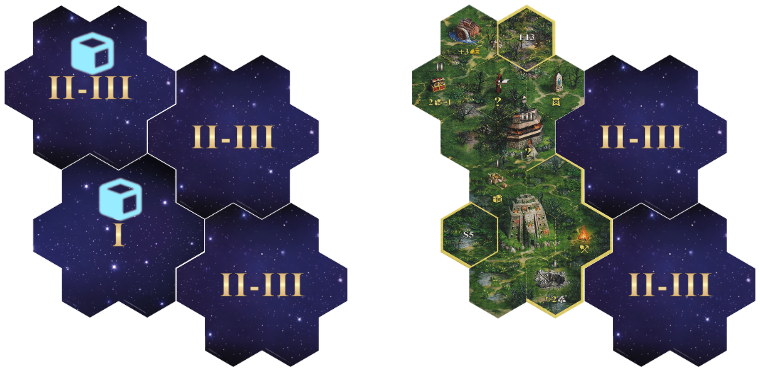
\includegraphics[width=0.68\paperwidth]{\maps/close_to_enemies_p1.png}
  \end{figure}
%   \vspace{2em}
  \begin{figure}[h!]
    \centering
    \captionof{figure}{\textbf{2-PLAYER SCENARIO | EXAMPLE }}
    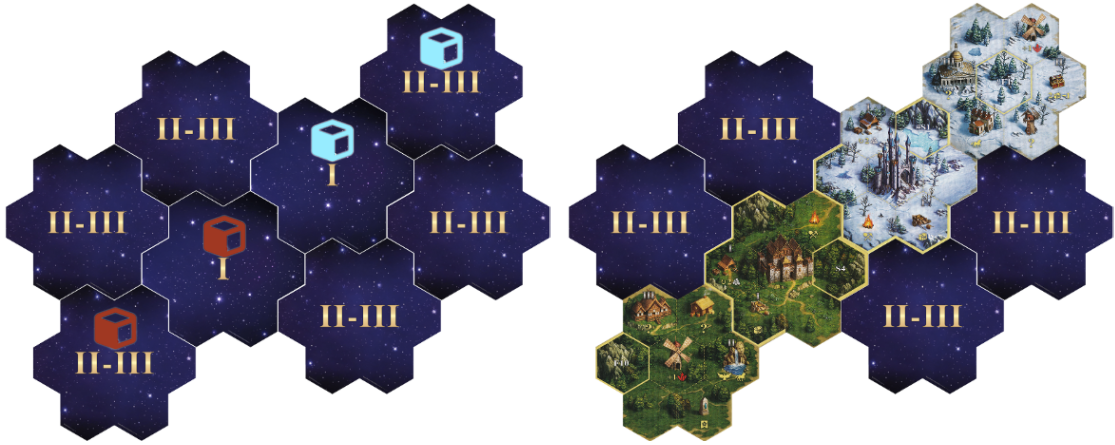
\includegraphics[width=0.68\paperwidth]{\maps/close_to_enemies_p2.png}
  \end{figure}
%   \vspace{2em}
  \begin{figure}[h!]
    \centering
    \captionof{figure}{\textbf{3-PLAYER SCENARIO | EXAMPLE}}
    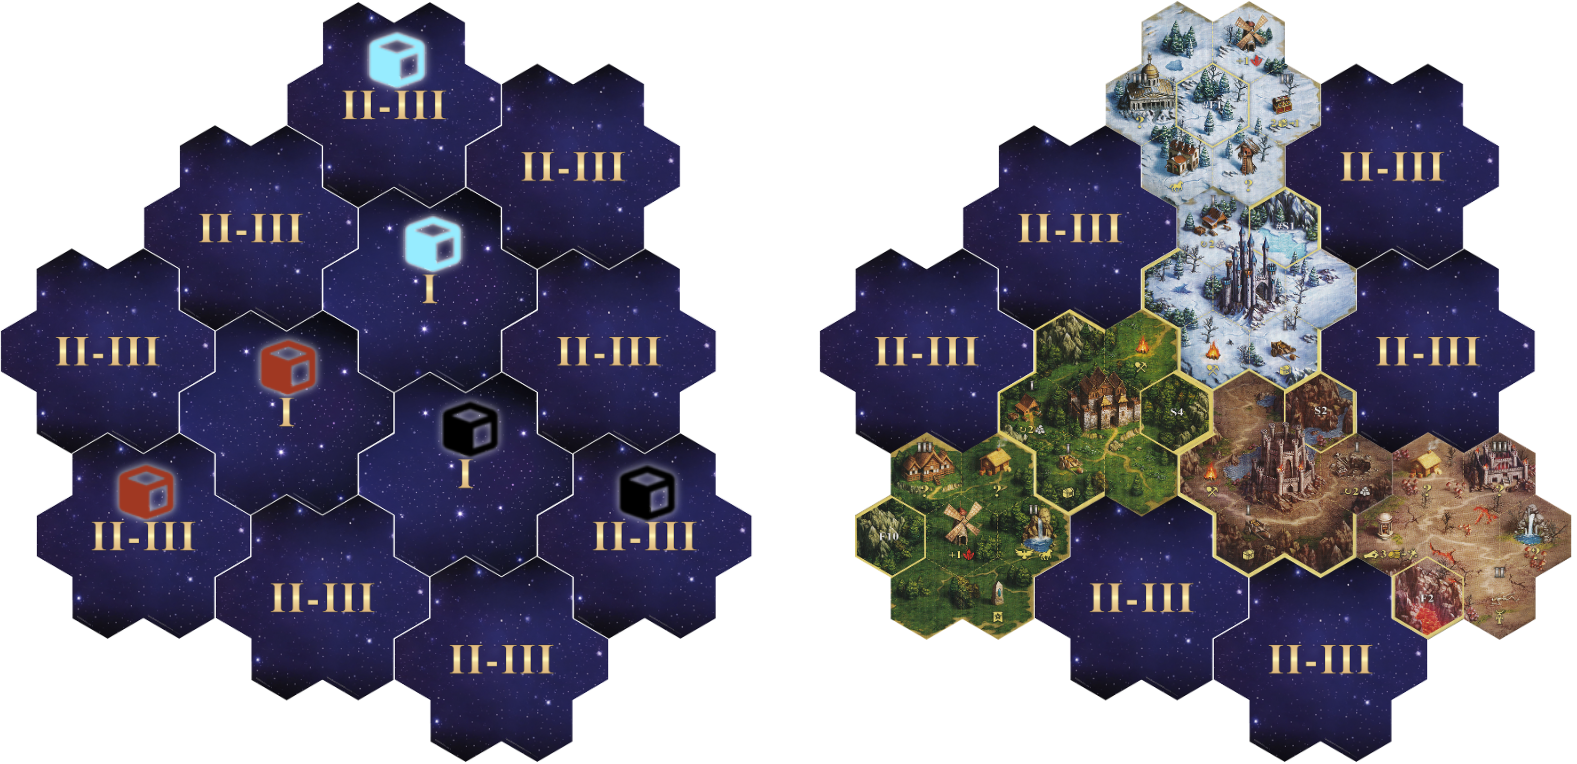
\includegraphics[width=0.75\paperwidth]{\maps/close_to_enemies_p3.png}
  \end{figure}
%   \vspace{2em}
  \begin{figure}[h!]
    \centering
    \captionof{figure}{\textbf{4-PLAYER SCENARIO | EXAMPLE}}
    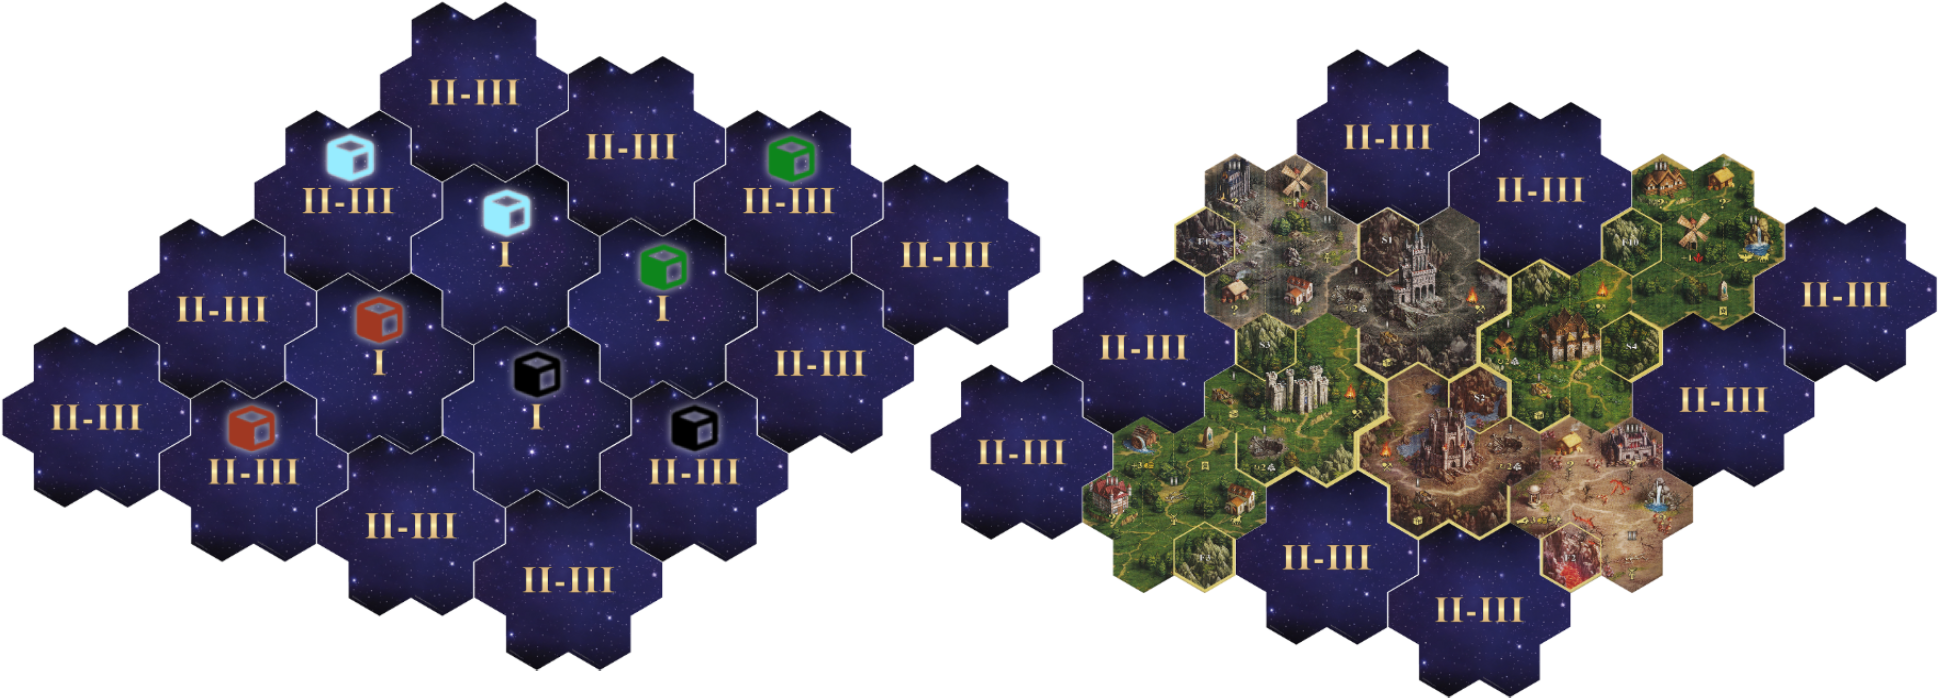
\includegraphics[width=0.85\paperwidth]{\maps/close_to_enemies_p4.png}
  \end{figure}
%   \vspace{2em}
  \begin{figure}[h!]
    \centering
    \captionof{figure}{\textbf{5-PLAYER SCENARIO | EXAMPLE}}
    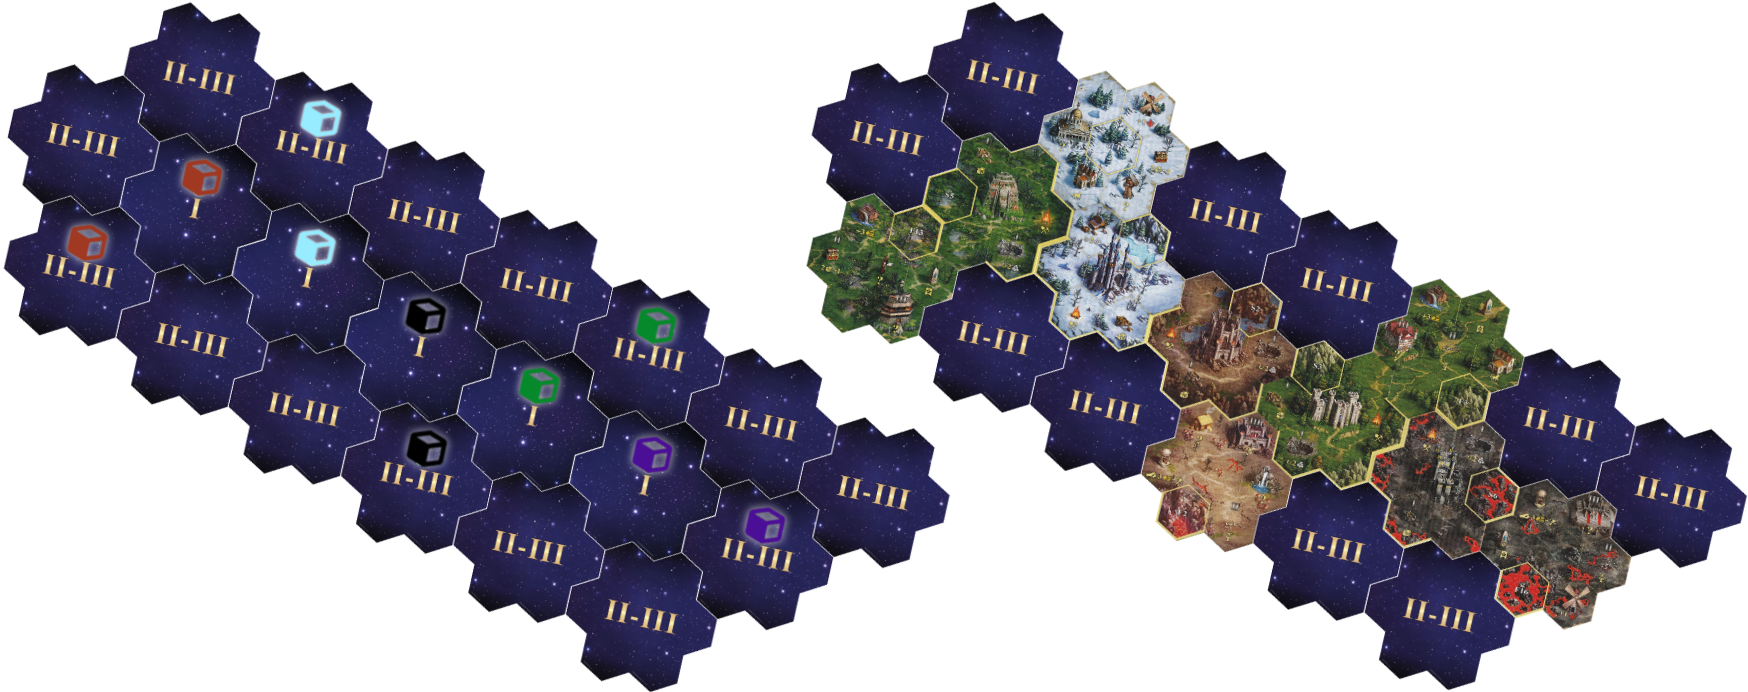
\includegraphics[width=0.75\paperwidth]{\maps/close_to_enemies_p5.png}
  \end{figure}
%   \vspace{2em}
  \begin{figure}[h!]
    \centering
    \captionof{figure}{\textbf{6-PLAYER SCENARIO | EXAMPLE}}
    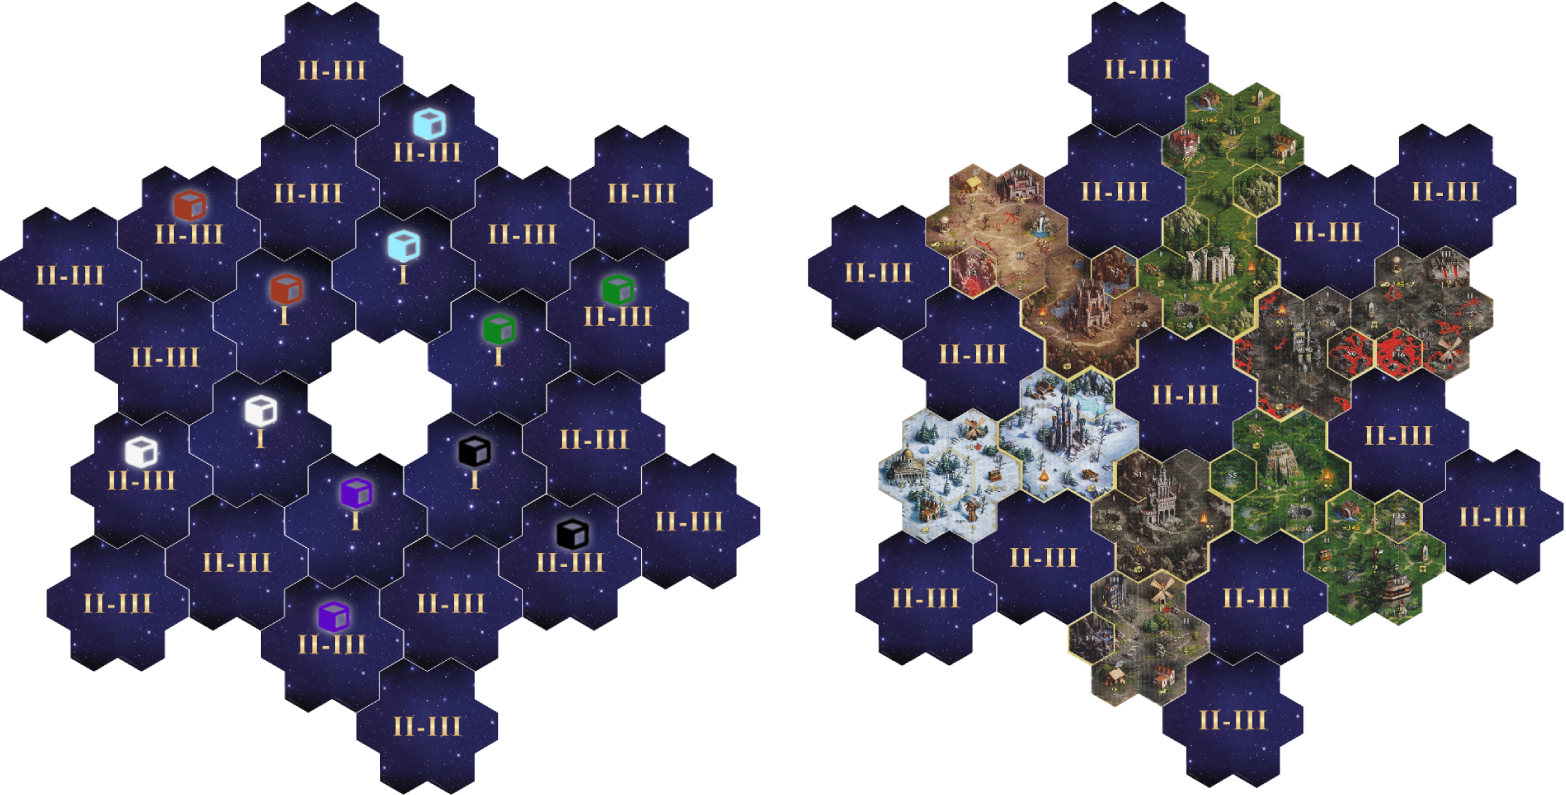
\includegraphics[width=0.75\paperwidth]{\maps/close_to_enemies_p6.png}
  \end{figure}

\end{center}
